\documentclass{amsart}
\usepackage{amsfonts, amsthm, amssymb, amsmath}
\usepackage{mathtools}
\usepackage{graphicx,caption,subcaption}
\usepackage{comment}
\usepackage{xcolor}
\usepackage{tikz}
%\usetikzlibrary{decorations.markings,arrows.meta,calc,fit,quotes,cd,math,external}
\usetikzlibrary{
  matrix,
  arrows,
  arrows.meta,
  calc,
  fit,
  quotes,
  cd,
  math,
  external,
  shapes,
  decorations.markings,
  decorations.pathreplacing,
  patterns,
  decorations.pathmorphing
}

\usepackage{url}
\usepackage[inline]{enumitem}
	\setlist{itemsep=0em, topsep=0em, parsep=0em}
	\setlist[enumerate]{label=(\alph*)}
\usepackage[all,2cell]{xy}\UseAllTwocells\SilentMatrices
\usepackage[breaklinks=true]{hyperref}%John's choices, can change; previous choice \definecolor{hyperrefcolor}{rgb}{0,0,0.7}
\definecolor{darkgreen}{rgb}{0,0.45,0}
\definecolor{myurlcolor}{rgb}{0.6,0,0}
\definecolor{mycitecolor}{rgb}{0,0,0.8}
\definecolor{myrefcolor}{rgb}{0,0,0.8}
\hypersetup{colorlinks, linkcolor=myrefcolor, citecolor=darkgreen, urlcolor=myurlcolor,
final,linktoc=page}
\usepackage[capitalize]{cleveref}
\crefname{equation}{}{}
\crefname{item}{}{}
\crefname{prop}{Proposition}{Propositions}

%
% environments and counters
%

\newtheorem{thm}{Theorem}[section]
\newtheorem{cnj}[thm]{Conjecture}
\newtheorem{lem}[thm]{Lemma}
\newtheorem{prop}[thm]{Proposition}
\newtheorem{cor}[thm]{Corollary}

\theoremstyle{remark}
	\newtheorem{remark}[thm]{Remark}
	\newtheorem{notation}[thm]{Notation}

\theoremstyle{definition}
	\newtheorem{ex}[thm]{Example} 
	\newtheorem{defn}[thm]{Definition}

% math text formatting
\newcommand{\cat}[1]{\mathsf{#1}}

% common category names

\newcommand{\Set}{\cat{Set}}
\newcommand{\Grph}{\cat{Grph}}
\newcommand{\Cat}{\cat{Cat}}
\newcommand{\twoCat}{\cat{2Cat}}
\newcommand{\Adj}{\cat{Adj}}
\newcommand{\one}{\mathbf{1}}
\newcommand{\two}{\mathbf{2}}
\newcommand{\Fib}{\cat{Fib}}
\newcommand{\OpFib}{\cat{OpFib}}
\newcommand{\Corefl}{\cat{Corefl}}
\newcommand{\Rali}{\cat{Rali}}

\newcommand{\C}{\cat{A}}
\newcommand{\D}{\cat{X}}
\newcommand{\A}{\cat{A}}
\newcommand{\X}{\cat{X}}
\newcommand{\U}{U}
\newcommand{\Q}{Q}
\renewcommand{\L}{L}
\newcommand{\R}{R}
\renewcommand{\P}{P}
\newcommand{\B}{\cat{B}}
\newcommand{\Y}{\cat{Y}}

\newcommand{\Cocart}{\mathrm{Cocart}}
\newcommand{\Cart}{\mathrm{Cart}}

\newcommand{\op}[1]{\operatorname{#1}}
\renewcommand{\t}[1]{\text{#1}}

\newcommand{\from}{\colon}
\newcommand{\xto}[1]{\xrightarrow{#1}}
\newcommand{\To}{\Rightarrow}
\newcommand{\Tto}{\Rrightarrow}
\newcommand{\bydef}{\coloneqq}
\newcommand{\define}{\textbf}%consider change to bold? or something else?

%
% math operators
%

\DeclareMathOperator{\Hom}{Hom}
\DeclareMathOperator{\id}{id}
\DeclareMathOperator{\ob}{Ob}
\DeclareMathOperator{\arr}{arr}
\DeclareMathOperator{\im}{im}
\DeclareMathOperator{\Aut}{Aut}
\DeclareMathOperator{\Bij}{Bij}
\DeclareMathOperator{\Sub}{Sub}
\DeclareMathOperator{\colim}{colim}
\newcommand{\iso}{\cong}

%
% tikz styles
%

% arrows for commuting diagram
\tikzset{
  cd/.style={
    ->,
    scale=6,
    >=angle 90,
    font=\scriptsize}
  }

% its us!

\definecolor{purple(x11)}{rgb}{0.5, 0.0, 0.5}
\newcommand{\chris}{\color{purple(x11)}}
\newcommand{\daniel}{\color{red}}

\begin{document}
\title{A note on Fibrations and Adjunctions}

\author{Daniel Cicala and Christina Vasilakopoulou} 
\address{update departments}
\email{update emails}

\begin{abstract}
Fibrations and Adjunctions rock.
\end{abstract}

\maketitle
% \tableofcontents


% ===============================================================
% Introduction

% ===============================================================
% Preliminaries. Basic def's and set notation. Include lemmas

\section{Preliminaries}\label{sec:preliminaries}

In this section, we present the necessary background for this paper
and take this opportunity to set our notation and conventions. One
convention we employ is the singular focus on opfibrations instead of
their dual, fibrations.  We specifically cover two flavors of
opfibrations: Grothendieck and Street.  We also present, for each type
of opfibration, a helpful lemma that relates colimits in the fibres to
colimits in the total category.

\subsection*{Grothendieck Opfibrations}

We recall some basic material from the theory of (Grothendieck) opfibrations; standard references include \cite{Handbook2,Grayfibredandcofibred,hermidaphd}. 

Consider a functor $\U \colon\X \to \A$. A morphism $\beta \colon x \to y$ in $\X $ over a morphism $f = \U(\beta) \colon a \to b$ in $\A$ is called \define{cocartesian} if and only if, for all $g \colon b \to b'$ in $\A$ and $\gamma \colon x\to y'$ in $\X $ with $\U(\gamma) = g\circ f$, there exists a unique $\delta \colon y\to y'$ in $\X$ such that $\U(\delta) = g$ and $\gamma = \delta \circ \beta$:
\begin{equation}\label{eq:opfibration}
\xymatrix @R=.1in @C=.6in
{&& y'\ar @{.>}@/_/[dd] &&\\
x\ar[r]_-{\beta} \ar @{.>}@/_/[dd]
\ar[urr]^-{\gamma} & 
y \ar @{.>}@/_/[dd] \ar @{-->}[ur]_-{\exists! \delta}
&& \textrm{in }\X\\
&& b' &&\\
a\ar[r]_-{f=\U\beta} \ar[urr]^-{g\circ f=\U\gamma}
 & b \ar[ur]_-g && \textrm{in }\A}
\end{equation}
For any object $a\in\A$, we denote by $\X_a$ the \define{fibre} of $U$ over $a$, i.e. the subcategory of $\X$ which consists of objects $x$ above $a$, namely $\U(x) = a$, and vertical morphisms $\beta$, namely $\U(\beta) = 1_a$. The functor $\U \colon \X \to \A$ is an \define{opfibration} if and only if, for all $f \colon a \to b$ in $\A$ and $x\in\X_a$, there is a cocartesian morphism $\beta$ with domain $x$ above $f$; it is called a \define{cocartesian lifting} of $b$ along $f$. The category $\A$ is called the \define{base} of the opfibration, and $\X $ its \define{total category}.
Of course, this is a dual notion to that of a \define{fibration}.

For any opfibration $\U\colon \X \to\A$, assuming the axiom of choice we may select a cocartesian arrow over each $f\colon a\to b$ in $\A$ and $x\in\X_a$, denoted by $\Cocart(f,x)\colon x\to f_!(x)$. Such a choice of cocartesian liftings is called a \define{cleavage} for $\U$, which is then called a \define{cloven opfibration}; in this way, any opfibration can be assumed to be cloven. As a special case of the universal property, any arrow in the total category of an opfibration factorizes uniquely into a cocartesian morphism followed by a vertical one:
\begin{equation}\label{factor}
\xymatrix @C=.6in @R=.3in
{x \ar @{.>}[dd]\ar[rr]^\gamma \ar[drr]_-{\Cocart(f,x)} && y &\\
&& f_!x \ar @{-->}[u]_-{\delta} \ar @{.>}[d] & \textrm{in }\X  \\
a\ar[rr]_-{f} && b & \textrm{in }\A.}
\end{equation}
The choice of cocartesian liftings in a cloven opfibration induces a so-called \define{reindexing functor} between the fibre categories
\begin{equation}\label{reindexing}
 f_!\colon\X_a\to\X_b
\end{equation}
for any $f\colon a\to b$ in the base category. It can be verified by the cocartesian lifting property that $(1_a)_!\cong1_{\X_a}$ and $(f\circ g)_!\cong f_!\circ g_!$. If these isomorphisms are equalities, we have the notion of a \define{split} (op)fibration.

For what follows, it is necessary to clarify the relation between the existence of colimits in the total category of an opfibration to the existence of those colimits in the fibres in a coherent way. For more details, and a proof of the following result, see \cite[Cor. 3.7]{FibredAdjunctions}.

\begin{lem}\label{lem:fibrewiselimits}
  Suppose $\cat{J}$ is a small category and $\U\colon\X\to\A$ is an
  opfibration whose base $\A$ has $\cat{J}$-colimits. The following
  are equivalent:
\begin{enumerate}
 \item all fibres have $\cat{J}$-colimits, and the reindexing functors preserve them; \label{it:2}
 \item the total category $\X$ has $\cat{J}$-colimits, and $\U$ strictly preserves them.
\end{enumerate}
\end{lem}
The above formulation and its dual version relate opfibrations specifically with colimits and fibrations with limits. Notice that condition \ref{it:2} is the usual formal definition of when an arbitrary opfibration has \emph{opfibred $\cat{J}$-colimits}, which in principle does not require a $\cat{J}$-cocomplete base. The strict preservation of colimits is discussed in detail in Appendix \ref{lem:isofactid}.

\subsection*{Street Opfibrations}

Typically, constructions in category theory should transport across equivalent categories. Opfibrations do not have this property. One can extend an opfibration $U\from\X\to\A$ along an equivalence of categories $\A \to \A'$ and the result $\X\to\A\to\A'$ is not necessarily an opfibration. The aspect that fails is, given a cocartesian lifting $\beta\from x \to y$ of an arrow $f\from a \to b$, we require that $Uy$ \emph{equals} $b$, and this equality may weaken to an isomorphism through an equivalence of categories. Street opfibrations avoid this defect. They were originally defined internally to 2-categories \cite{FibYon}. The definition below is a special case when the 2-category is $\Cat$.

\begin{defn}
  A functor $ U \from \X \to \A $ is a \define{Street
    opfibration} if, for any arrow $ f \from a \to b $ in $ \A
  $ and $ x $ above $ a $, there exists a
  cocartesian arrow  $ \theta \from x \to y $ and an
  isomorphism $ h \from b \iso Uy $ such that $ fh = U\theta $.
\end{defn}

There is no amended definition of ``cocartesian arrow'' here; it is the same as above. It is the isomorphism $ h $, which replaces an equality in a Grothendieck opfibration, that ensures Street opfibrations satisfy the priciple of equivalence.

Because we generalize our results in Section \ref{sec:groth-fibs-ralis} from Grothendieck fibrations to Street fibrations, we need a generalized version of Lemma \ref{lem:fibrewiselimits}. In order to do this, we present several standard results as lemmas and recall the definition of an isofibration.

\begin{defn}
  A functor $U \from \X \to \A$ is an \define{isofibration} if, for every isomorphism $f \from Ux \to a$ in $\A$, there is an isomorphism $\hat{f} \from x \to x'$ in $\X$ such that $U\hat{f}=f$. 
\end{defn}

\begin{lem}
  If a functor is a Street opfibration and isofibration, it is also a Grothendieck fibration. 
\end{lem}

\begin{proof}
  Let $U \from\X \to \A$ be both a Street opfibration and isofibration. To an arrow $f \from Ux \to a$, we associate an opcartesian lifting $\theta \from x \to y$ and isomorphism $h \from a \to Uy$. Let $\hat{h^{-1}}$ be the invertible arrow in $\X$ over $h^{-1}$. The cocartesian arrow lift of $f$ is $\theta \hat{h^{-1}}$.  
\end{proof}

\begin{lem}
  A Street opfibration can be decomposed into a Grothendieck opfibration followed by an equivalence of categories.
\end{lem}

\begin{proof}
  There is a model structure on $\Cat$ whose weak equivalences are equivalences of categories and fibrations are isofibrations \cite{rezk}. Hence, we can decompose a Street opfibration into an isofibration followed by a equivalence of categories. But because the isofibration is equivlant to a Street opfibration, it is also a Street opfibration, hence a Grothendieck opfibration by the previous lemma.  
\end{proof}


\begin{lem} \label{lem:street-fibrewise-limits}
  Suppose $ \cat{J} $ is a small category and $ U \from \X
  \to \A $ is a Street opfibration. If $ \A $ has $ \cat{J}
  $-colimits, the following are equivalent:
  \begin{enumerate}
  \item
    all fibres have $ \cat{J} $-colimits and the
    reindexing functors preserve them;
  \item
    $ \X $ has $ \cat{J} $-colimits and $ U $ preserves
    them.
  \end{enumerate}
\end{lem}

\begin{proof}
  Decompose $U$ into a Street opfibration $U' \from \X \to \A'$ followed by an equivalence $H \from \A' \to \A$ per the previous lemma.  If the $U$-fibres have have $\cat{J}$-colimits, then so do the equivalent $U'$-fibres.  But then by Lemma \ref{lem:fibrewiselimits}, $\X$ has $\cat{J}$-colimits and $U'$ strictly preserves them, which ensures that $U$ preserves them.  

  \daniel{pick up here with 'only if' direction. Think: U preserves colimits implies U' strictly?  U' strictly even needed in grothendieck case?}


  Every Street fibration can be factored as a Grothendieck fibration
  followed by an equivalence of categories. {\chris a reference is
    necessary here, and a diagram expressing that property could go
    here or earlier, discussing the relation of this new notion with
    the old.} This lemma holds for Grothendieck fibrations plus
  categories having colimits and functors preserving them are both
  properties that satisfy the principle of equivalence.
\end{proof}

\subsection*{Coreflections and laris}

The main result of this paper is a correspondence between fibrations and adjoints, under certain assumptions. The adjunctions involved are a stricter version of the well-known \emph{coreflections}, whose definition we recall. %if we need ref for this super standard thing, Borceaux 1

\begin{prop}\label{prop:coreflection}
The following are equivalent for an adjunction $\L\dashv\U\colon\X\to\A$:
 \begin{enumerate}
  \item the left adjoint $\L$ is fully faithful;
  \item the unit $\eta\colon1_\A\Rightarrow \U\L$ is an isomorphism.
 \end{enumerate}
Under these conditions, $\U\epsilon$ and $\epsilon_\L$ are also isomorphisms.
\end{prop}

The above clauses also imply that the induced comonad $(LU,L\eta_G,\epsilon)$ on $\X$ is \emph{idempotent}. Such an adjunction is called a \define{coreflection}, $\A$ is a \define{coreflective} subcategory of $\U$ and the right adjoint $U$ is called the \define{coreflector}.

Connected to the issues of `evilness' discussed already is a stricter version of a coreflector that actually appears in the desired correspondence between (Gro\-the\-ndi\-eck) fibrations and adjoints.
We use the acronym \emph{lari}, originally introduced in~\cite{Grayfibredandcofibred}, for the notion of a `left adjoint, right inverse' functor. Explicitly, if $\U\colon\X\to\A$ has a lari $\L$, then $\L\dashv \U$ and $\eta\colon1_\A=\U\L$. Equivalently, in this case we can say that $\U$ is a \emph{rali}, namely it is a right adjoint, left inverse of some $\L$ --- still the unit of the adjunction is the identity, with $\U$ now being a left inverse. Of course, under these conditions, $\U\epsilon$ and $\epsilon_\L$ are also identities $ULU=U$.

Analogously, if a functor has a \emph{rari} or equivalently is a \emph{lali}, then the counit of the adjunction is the identity; this comes as a special case of the dual notion of a \emph{reflection} of categories.

{\chris Either here or in section 5}

Recall that a \emph{map of adjunctions} $(F,G)\colon(L\dashv U)\to(L'\dashv U')$ is given by two functors $F$ and $G$ that make both squares below commute 
%again, for reference for this super standard thing, MacLane.
\begin{displaymath}
\begin{tikzcd}[sep=.6in]
\X\ar[d,bend left,"U"]\ar[r,"F"]\ar[d,phantom,"\dashv"description] & \X'\ar[d,bend left,"U'"]\ar[d,phantom,"\dashv"description] \\
\A\ar[u,bend left,"L"]\ar[r,"G"'] & \A'\ar[u,bend left,"L'"] \\
\end{tikzcd}
\end{displaymath}
and moreover $G\eta=\eta'_{G}$ (or equivalently $\epsilon'_{F}=F\epsilon$).
{\chris Not sure if we should go 2-categorical after all. Haven't ever heard of 2-cells between maps of adjunctions. Leave out for now.}

We obtain a category $\Adj$ with objects pairs {\chris we need to decide if the adjoint is part of the object, probably yes} of adjoint functors $(L,U)$ and morphisms maps of adjunctions between them. Moreover, there is a full subcategory $\Corefl$ of coreflections, as well as a full subcategory $\Rali$ of adjunctions whose right adjoint is left inverse (equivalently, whose left adjoint is right inverse). Notice that for the morphisms of the latter, the condition $G\eta=\eta'_{G}$ is automatically satisfied since the unit is the identity.

% ===============================================================
% Groth fibs and ralis. Examine relationship between.

\section{Grothendieck fibrations and ralis}
\label{sec:groth-fibs-ralis}

In this section, we investigate conditions under which opfibrations and adjunctions with identity unit relate to one another. The main result, \cref{thm:mainthm}, exhibits their bijective correspondence under the intersection of the respective conditions.

Initially we establish when an opfibration has a left adjoint; the following result is the dual of \cite[Prop. 4.4]{Grayfibredandcofibred}.

%changed from has a lari to is a rali to make descriptions of categories easier later - hopefully! Otherwise change back.
\begin{prop} \label{prop:opfibtolari}
  Let $\U \from \D \to \C$ be an opfibration. Then
  $\U$ is a rali if (and only if) its fibers have
  initial objects which are preserved by the
  reindexing functors.
\end{prop}

\begin{proof}
Denote by $\bot_a$ the initial object in each fiber $\D_x$ above an object $a\in\C$ in the base category. Define a left adjoint $\L$
of $\U$ as follows:
\begin{displaymath}
\begin{tikzcd}[row sep=.05in,cells={anchor=east}]
  \L\colon\A\ar[rr] && \X\;\; &\\
  a\ar[rr,mapsto]\ar[dd,"f"'] && \bot_a\ar[dd,dashed,"\L f"']\ar[ddr,"{\Cocart(f,\bot_a)}"] & \\
\hole \\
b\ar[rr,mapsto] && \bot_b & f_!(\bot_a)\ar[l,"\sim"']
\end{tikzcd}
\end{displaymath}
where the bottom isomorphism is the unique one
induced by the fact that each $f_!$ preserves
initial objects between the respective
fibers.
% looks like the first time we define a
% morphism in the total category via its
% unique factorization! alright.
This assignment is strictly functorial due to the
universal properties of cocartesian
liftings. Notice that by definition,
$\L a =\bot_a$ is in the fibre $\X_a$, which means
$\U\L a =a$ for any object $a\in\A$.

To show this determines a left adjoint of $\U$, it
suffices to establish a natural bijection
$\X(\L a,x)\cong\A(a,\U x)$ for any $a\in\A$,
$x\in\X$. Indeed, each morphism in the total
category $k\colon \L a\to x$ above $f=\U k$,
factorizes uniquely \cref{factor} as
\begin{displaymath}
\xymatrix @C=.5in @R=.3in
{\bot_a \ar @{.>}[dd]\ar[rr]^k \ar[drr]_-{\Cocart(f,\bot_a)} && x &\\
&& f_!(\bot_a) \ar @{-->}[u]_-s \ar @{.>}[d] & \textrm{in }\X \\
a\ar[rr]_-{f} && \U x & \textrm{in }\A}
\end{displaymath}
but since $f_!(\bot_a)\cong\bot_{\U x}$ is the initial object in the fibre above $\U x$, the morphism $s$ is in fact unique. As a result, every $k$ uniquely corresponds to some $f$ in that way, and this isomorphism is natural.

Finally, the right adjoint $\U$ is indeed a left
inverse of $\L$, namely the unit of the adjunction
$\eta\colon 1_\A \to \U\L$ is the identity natural
transformation: $\U\L a=a$ and moreover $\X (\L a,\L a)\cong\A(a,\U\L a)$ ensures that the identity $\bot_a$ corresponds to the identity on $a$. %which should be clear from the above described bijection!
\end{proof}

The `only if' direction of the statement is not needed for our purposes. Notice that in particular, since $\U$ is a right adjoint, it ends up preserving all limits that exist in $\X$; this makes the above condition for its existence look slightly unintuitive. 

The dual result states that a fibration is a lali, or equivalently has a rari namely the counit of the adjunction is the identity, if and only if the fibers have terminal objects that are preserved by the reindexing functors. Due to \cref{lem:fibrewiselimits}, we can express both these results as follows.

\begin{cor}
An (op)fibration is a (right) left adjoint left inverse if the base category has and the functor strictly preserves the (initial) terminal object.
\end{cor}

Next, we examine when a right adjoint left inverse has an opfibration structure. The relevant colimits in this case are pushouts, and the following result provides sufficient conditions in terms of those. Recall the discussion regarding strict preservation of colimits in \cref{sec:preliminaries}.

\begin{prop}\label{prop:laritoopfib}
Suppose that $\U\colon\X\to\A$ is a rali, with left adjoint right inverse $\L$. Then $\U$ is an opfibration if $\X$ and $\A$ have chosen pushouts such that $\U$ strictly preserves them.
\end{prop}

\begin{proof}
First of all, suppose that the rali $\U\colon\X\to\A$ preserves pushouts, which are chosen such that pushouts  of a morphism along an identity is the morphism itself. We will show it has the structure of a cloven Grothendieck opfibration. Indeed, take a morphism $f\colon a\to b$ in $\A$ and an object $x\in\X$ above $a$, as in
\begin{displaymath}
\xymatrix @C=.5in @R=.3in
{x \ar @{.>}[d]_-{\U} &&& \textrm{in }\X \\
a\ar[rr]_-{f} && b & \textrm{in }\A .}
\end{displaymath}
Define the cocartesian lifting of $x$ along $f$ to be the horizontal dashed arrow to the (chosen) pushout of the following diagram in $\X$ 
\begin{displaymath}
 \begin{tikzcd}
   \L\U x\ar[r,"\L f"]\ar[d,"\varepsilon_a"'] & \L b\ar[d,dashed] \\
   x\ar[r,dashed] & x+_{\L\U x} \L b
 \end{tikzcd}
\end{displaymath}
where $\varepsilon\colon \L\U\Rightarrow1_\X$ is the counit
of the adjunction $\L\dashv \U$. To verify this is a cocartesian lifting, first of all it must be mapped to
$f$ via $\U$: if we apply $\U$ to the above
square, using the facts that
$\U\varepsilon_x=1_{a}$, $\U\L f=f$ (by \cref{prop:coreflection}) and
$$\U (x+_{\L\U x}\L b)=\U x+_{\U\L\U x}\U\L b =
a+_{a} b $$ since $\U$ strictly preserves pushouts, the
resulting colimit diagram 
\begin{displaymath}
 \begin{tikzcd}
  a\ar[r,"f"]\ar[d,"1_a"'] & b\ar[d,dashed] \\
a\ar[r,dashed] & a+_{a}b=b
 \end{tikzcd}
\end{displaymath}
is \emph{the} pushout of $f$ along the identity, namely $f$ due to our choice. Moreover, the universal property \cref{eq:opfibration} of the proposed cocartesian lifting follows from universality of pushouts thus the one direction of the proof is complete.
\end{proof}
%Christina: tried to see whether the converse is true, didn't go far. Remember that from previous prop we got it preserves initial for sure!

Combining \cref{prop:opfibtolari,prop:laritoopfib}, we obtain the following result that establishes certain conditions under which a Grothendieck opfibration structure on a functor corresponds to a rali structure and vice versa. %Christina: no more finite colimits: Steve said that for the strict case, this is more subtle than the ordinary case. Pretty sure that we don't wanna go into details there?
%Understand whether other such conditions could exist? More philosophically.

\begin{thm}\label{thm:mainthm}
Suppose that $\X$ and $\A$ have chosen pushouts and initial objects, and a functor $\U\colon\X\to\A$ strictly preserves them. Then $\U$ is a right adjoint left inverse if and only if $\U$ is an opfibration.
\end{thm}

% ===============================================================
% Street fibs and corefls. Examine relationship between.

\section{Street fibrations and coreflections}\label{Streetfibs}

In this section, we trod the same path as in Section
\ref{sec:groth-fibs-ralis} yet shed all strictness of the
preservation of colimits and work with Street opfibrations
instead of Grothendeick opfibrations.

Generalising \cref{prop:opfibtolari}, we obtain
the following. 

\begin{prop}
  \label{thm:street-opfib-to-corefl}
  Let $ \U \from \X \to \A $ be a Street
  opfibration. Then $ \U $ is a coreflector if its
  fibers have initial objects which are preserved
  by the reindexing functors.
\end{prop}

\begin{proof}
  We define $ \L $ exactly as in Proposition
  \ref{prop:opfibtolari}. 

  The unit of the adjunction $ \L \dashv \U $ is the
  identity $ a\to \U\L a = \U\bot_a = a $.  The
  counit is the initial map $ \bot_{\U x} = \L\U x \to
  x $.  The triangle identities are satisfied as
  well. The first is the composite
  \[
    \L a
    \xto{\L\eta_a}        \L\U\L a
    \xto{\epsilon_{\L a}} \L a
  \]
  which is given by $ \bot_a \to \bot_a \to \bot_a
  $.  The second is the composite
  \[
    \U x
    \xto{\eta_{\U x}} \U\L\U x
    \xto{\U\eta_x}    \U x
  \]
  which is given by $ \U x \to \U x \to \U x $.

  Because the unit of the adjunction is an
  isomorphism, $ \L $ is full and faithful
  \cite[{Prop.~1.3}]{gabrielzisman} making $ \U $ a
  coreflector.
\end{proof}

Applying Lemma \ref{lem:street-fibrewise-limits}, we can
transport the assumptions on the fibers to the base category
of our Street fibration.

\begin{cor}
  A Street (op)fibration is a coreflector if the base
  category has and the functor preserves the (initial)
  terminal object.
\end{cor}

Generalising \cref{prop:laritoopfib}, we obtain the following result.

\begin{prop}
  \label{thm:corefl-to-street-opfib}
  Suppose that $ \U \from \X \to \A $ is a
  coreflector. Then $ \U $ is a Street opfibration
  if $ \X $ has pushouts and $ \U $ preserves them.
\end{prop}

\begin{proof}
  Fix an arrow $ f \from a \to b $ in $ \A $
  and an object $ x $ in the fibre of $ a $. We
  claim that $ \hat{f} $, defined as the pushout
  of $ \L f $
  along the counit $ \epsilon_x $
  \[
    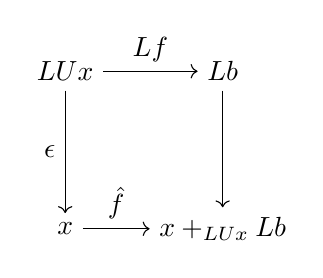
\begin{tikzpicture}
      \node (ul) at (0,2) {$ \L \U x $};
      \node (ll) at (0,0) {$ x $};
      \node (ur) at (2,2) {$ \L b $};
      \node (lr) at (2,0) {$ x +_{\L\U x} \L b$};
      \draw [->] (ul) to node [left] {$ \epsilon $} (ll);
      \draw [->] (ul) to node [above] {$ \L f $} (ur);
      \draw [->] (ll) to node [above] {$ \hat{f} $} (lr);
      \draw [->] (ur) to (lr);
    \end{tikzpicture}
  \]
  is the cocartesian lift. There is a string of
  isomorphisms
  \[
    \U ( x +_{\L\U x} \L b ) \cong
    \U x +_{\U\L\U x} \L b \cong
    \U x +_{\U x} b \cong
    b
  \]
  whose composite we call $ h $.  Then
  \[
    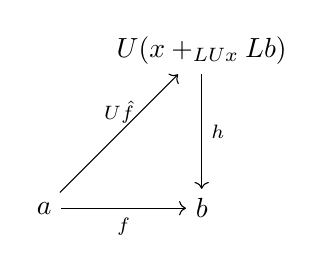
\begin{tikzpicture}
      \node (a) at (0,0) {$ a $};
      \node (b) at (2,0) {$ b $};
      \node (c) at (2,2) {$ \U ( x+_{\L\U x} \L b ) $};
      \path[->,font=\scriptsize]
      (a) edge node[below]{$ f $} (b)
      (a) edge node[above]{$ \U\hat{f} $} (c)
      (c) edge node[right]{$ h $} (b);
    \end{tikzpicture}
  \]
  commutes, and so $ \hat{f} $ is an appropriate
  lift. It remains to show that $ \hat{f} $ is
  cocartesian.

  Consider a $ \X $-arrow $ g \from x \to y $
  with a $ \A $-arrow
  $ \theta \from \U( x +_{\L\U x} \L b ) \to \U y $ so
  that $ \theta \U \hat{f} = \U g $.  Can we
  uniquely lift $ \theta $? Set up the diagram
  \[
    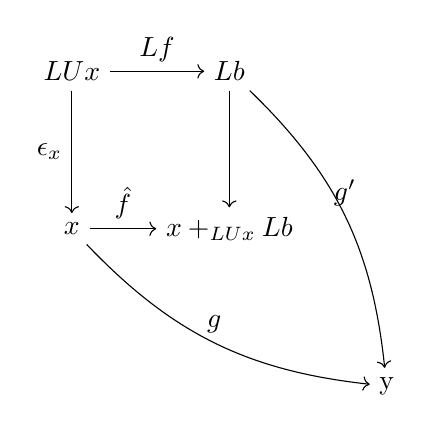
\begin{tikzpicture}
      \node (ul) at (0,2) {$ \L\U x $};
      \node (ll) at (0,0) {$ x $};
      \node (ur) at (2,2) {$ \L b $};
      \node (lr) at (2,0) {$ x +_{\L\U x} \L b$};
      \node (comp) at (4,-2) {y};
      \draw [->] (ul) to node [left] {$ \epsilon_x $} (ll);
      \draw [->] (ul) to node [above] {$ \L f $} (ur);
      \draw [->] (ll) to node [above] {$ \hat{f} $} (lr);
      \draw [->] (ur) to (lr);
      \draw [->] (ll) to [bend right=20] node [above] {$ g $} (comp);
      \draw [->] (ur) to [bend left=20] node [above] {$ g' $} (comp);
    \end{tikzpicture}
  \] 
  where $ g' \bydef \epsilon_y \L\theta \L h^{-1} $.
  To show the outer square commutes, it suffices
  to show that $ g' \L f $ and $ g \epsilon_x $
  have the same image under the adjunction homset
  correspondence.  We have
  \[
    g' \circ \L f =
    \epsilon_y \circ \L\theta \circ \L h \circ \L f
    \mapsto
    \U\epsilon_y \circ \U\L\theta \circ \U\L h
      \circ \U\L f \circ\eta_{ux}
    = \theta \circ h \circ f   
    = \theta \circ \U \circ \hat{f} 
    = \U g
  \]
  and 
  \[
    g \epsilon_x
    \mapsto
    \U g \circ \eta_{\U x}
    = \U g
  \]
\end{proof}

We now intersect the hypothesis of Propositions
\cref{thm:street-opfib-to-corefl} and
\cref{thm:corefl-to-street-opfib} to provide the
main result of this section.

\begin{thm}
  \label{thm:main-theorem-street-version}
  Let $ U \from \X \to \A $ be a functor such that $ \A $
  and $ \X $ have chosen initial objects and pushouts and
  $ U $ preserves them. Then $ \U $ is a coreflector if and
  only if $ \U $ is a Street opfibration.
\end{thm}

% ===============================================================
% Cats of fibs and adjs. Examine structure of relationship (todo later)



% ===============================================================
% Appendix. Choice of colimits.

\appendix{}

\section{Choice of colimits}

In what follows, and in particular for our main \cref{thm:mainthm}, we often require that certain colimits must be \emph{strictly} preserved. Although the strict preservation of colimits does not adhere to the principle of equivalence, it is required when working with Grothendieck fibrations. Moreover, in \cref{Streetfibs} we examine the non-strict context which then naturally matches to the notion of a Street fibration as discussed above.

In more detail, assuming the axiom of choice we can regard any category with colimits as having \emph{chosen} ones, in the sense of choosing a specific adjoint (from all isomorphic ones) to the constant diagram functor:
\begin{displaymath}
 \begin{tikzcd}[sep=.7in]
 \cat{C}\ar[r,pos=.6,"\Delta_\cat{C}"description]\ar[r,phantom,bend left=18,pos=.6,"\bot"]\ar[r,phantom,bend right=18,pos=.6,"\bot"] &  {[}\cat{J},\cat{C}{]}\ar[l,bend right,pos=.4,"\colim_\cat{J}"']\ar[l,bend left,pos=.4,"\lim_\cat{J}"]
 \end{tikzcd}
\end{displaymath}
Some categories, like $\Set$, even have a canonical choice corresponding to well-known constructions of colimits of sets. In general, a functor $F\colon\cat{C}\to\cat{D}$ between categories with colimits, for example, preserves them when the following diagram
\begin{equation}\label{eq:preservelimits}
  \begin{tikzcd}
\phantom{A}[\cat{J},\cat{C}]\ar[r,"\colim"]\ar[d,"{[\cat{J},F]}"']\ar[dr,phantom,"\cong"] & \cat{C}\ar[d,"F"] \\
\phantom{A}[\cat{J},\cat{D}]\ar[r,"\colim"'] & \cat{D}
  \end{tikzcd}
 \end{equation}
 commutes up to natural isomorphism.  The following two lemmas (due to
 Steve Lack) present two natural settings where functors between
 categories with chosen colimits strictly preserve them;
 evidently, such a thing is to be expected only when the colimits in the
 categories have been both previously constructed from chosen limits
 in some fixed category.
\begin{lem}\label{lem:Lack1}
 Suppose $\cat{C}$ is a category with chosen colimits of any class. Then for any two categories $\cat{A}$ and $\cat{B}$ and any functor $F\colon\cat{A}\to\cat{B}$ between them, the pre-composition functor
 \begin{displaymath}
  \begin{tikzcd}[row sep=.05in]
  F^*\colon[\cat{B},\cat{C}]\ar[r] & \;[\cat{A},\cat{C}] \\
  \;\;\;\;\left(\cat{B}\xrightarrow{H}\cat{C}\right)\ar[r,mapsto] & \left(\cat{A}\xrightarrow{F}\cat{B}\xrightarrow{H}\cat{C}\right)
  \end{tikzcd}
 \end{displaymath}
strictly preserves the chosen colimits.
\end{lem}
\begin{proof}
 This follows from the pointwise construction of colimits in functor categories.
\end{proof}

As a particular case, the following result concerns our motivating example.
\begin{cor}
There is a canonical choice of colimits in $\Grph$ inherited from those in $\Set$ so that the domain and codomain functors $\Grph\to\Set$ strictly preserve all colimits.
\end{cor}

\begin{proof}
  The domain and codomain functors, respectively $1^\ast$ and
  $2^\ast$, are built from the functors
  $1,2\colon\one{=}\{\bullet\}\longrightarrow\{1\rightrightarrows2\}{=}\two$.  Choosing the canonical colimits in $\Set$, by \cref{lem:Lack1} we obtain two functors
\begin{displaymath}
\begin{tikzcd}
 \Grph=[\two,\Set]\ar[r,shift left,"1^\ast"]\ar[r,shift right,"2^\ast"'] & \;[\one,\Set]=\Set
 \end{tikzcd}
\end{displaymath}
that strictly preserve them.
\end{proof}

The following case again follows from a construction of chosen limits in common ground; colimits adhere to a dual result.
\begin{lem}
Suppose $\cat{C}$ and $\cat{D}$ have chosen colimits and $F\colon\cat{C}\to\cat{D}$ is an arbitrary functor. Then the comma category $F\downarrow\cat{D}$ can be equipped with colimits in such a way that both projections $\cat{C}\leftarrow F\downarrow\cat{D}\to\cat{D}$ strictly preserve them.
\end{lem}

\begin{proof}
 This follows from the canonical construction of colimits in comma categories (see~\cite[\S 2.16]{Handbook1}).
\end{proof}

Finally, opfibrations form another class of functors that is notable when it comes to strictly preserving colimits. In more detail, we do not lose generality by assuming that a colimit preserving opfibration preserves strictly. Such a statement does not apply to arbitrary functors. This is due to the following lemma, which is a special case of a more general fact: the embedding of $\OpFib$ in the 2-category $\OpFib_{\sim}$ where 2-cells are squares filled with isomorphisms, is locally fully faithful and essentially surjective (also for fibs...references...\cite{Fib2Fib}?). We thank Claudio Hermida for these observations.
\begin{lem}\label{lem:isofactid}
 Suppose $\U$ and $\Q$ are opfibrations, and there is a natural isomorphism
 \begin{displaymath}
  \begin{tikzcd}
\X\ar[r,"H"]\ar[d,"\U"']\ar[dr,phantom,"\stackrel{\phi}{\cong}"] & \Y\ar[d,"\Q"] \\
\A\ar[r,"F"'] & \B
  \end{tikzcd}
 \end{displaymath}
Then $\phi$ factors as a commutative square composed by an isomorphism $\hat{\phi}$, as in
 \begin{displaymath}
  \begin{tikzcd}[row sep=.15in]
\X\ar[rr,bend left,"H"]\ar[rr,bend right,"\widehat{H}"']\ar[rr,phantom,"{\stackrel{\hat{\phi}}{\cong}}"description]\ar[dd,"\U"'] && \Y\ar[dd,"\Q"] \\
\hole \\
\A\ar[rr,"F"'] && \B
  \end{tikzcd}
 \end{displaymath}
\end{lem}
As a result, if $\U$ is an opfibration that preserves $\cat{J}$-colimits for some small $\cat{J}$, we can factor the natural isomorphism \cref{eq:preservelimits}, where the left leg is also a fibration, as
\begin{displaymath}
  \begin{tikzcd}[row sep=.15in]
{[\cat{J},\cat{X}]}\ar[rr,bend left,pos=.4,"\colim"]\ar[rr,bend right,pos=.4,"\widehat{\colim}"']\ar[rr,phantom,"\cong"description]\ar[dd,"{[\cat{J},\U]}"'] && \X\ar[dd,"\U"] \\
\hole \\
{[\cat{J},\cat{A}]}\ar[rr,"\colim"'] && \A
  \end{tikzcd}
 \end{displaymath}
essentially changing the choice of colimits in the total category and establishing that $Q$ now strictly preserves them. In a dual way, we may assume that any fibration strictly preserves chosen limits, if it preserves limits in the ordinary sense.



\bibliographystyle{plain}
\bibliography{references.bib}


\end{document}